\documentclass[10pt,aspectratio=169]{beamer}
\usepackage[utf8]{inputenc}
\usepackage[T1]{fontenc}
\usepackage[spanish,es-nodecimaldot]{babel}
\usepackage{lmodern}
\usepackage{amsmath,amssymb,bm,mathtools}
\usepackage{graphicx}
\usepackage{booktabs,tabularx,array,multirow}
\usepackage{ragged2e}
\usepackage{tikz}
\usetikzlibrary{arrows.meta,positioning,calc}
\usepackage{siunitx}
\graphicspath{{figures/}}

% Formato sobrio para presentación doctoral.
\usetheme{default}
\definecolor{navy}{RGB}{18,52,86}
\definecolor{slate}{RGB}{76,86,96}
\definecolor{rulegray}{RGB}{190,196,202}
\definecolor{lightgray}{RGB}{246,247,248}
\definecolor{textgray}{RGB}{35,39,43}
\setbeamercolor{normal text}{fg=textgray,bg=white}
\setbeamercolor{structure}{fg=navy}
\setbeamercolor{frametitle}{fg=navy,bg=white}
\setbeamercolor{title}{fg=navy,bg=white}
\setbeamercolor{subtitle}{fg=slate,bg=white}
\setbeamercolor{caption name}{fg=navy}
\setbeamercolor{footline}{fg=slate,bg=white}
\setbeamerfont{frametitle}{size=\large,series=\bfseries}
\setbeamerfont{caption}{size=\scriptsize}
\setbeamerfont{footline}{size=\tiny}
\setbeamertemplate{navigation symbols}{}
\setbeamertemplate{itemize item}{\raise0.2ex\hbox{\scriptsize$\blacksquare$}}
\setbeamertemplate{itemize subitem}{\raise0.2ex\hbox{\tiny$\blacktriangleright$}}
\setbeamertemplate{caption}[numbered]
\setbeamertemplate{frametitle}{%
  \vspace{0.18cm}\insertframetitle\par
  \vspace{0.06cm}{\color{rulegray}\rule{0.96\textwidth}{0.45pt}}
}
\setbeamertemplate{footline}{%
  \begin{beamercolorbox}[wd=\paperwidth,ht=2.5ex,dp=1.0ex,leftskip=0.75cm,rightskip=0.75cm]{footline}%
  A. G. Romero-Pacheco \hspace{0.7em}|\hspace{0.7em} Avances de tesis doctoral
  \hfill\insertframenumber/\inserttotalframenumber
  \end{beamercolorbox}
}
\setbeamersize{text margin left=0.75cm,text margin right=0.75cm}
\setlength{\tabcolsep}{4pt}
\renewcommand{\arraystretch}{1.12}

\newcommand{\vect}[1]{\bm{#1}}
\newcommand{\Hreal}{H^{\mathrm{real}}}
\newcommand{\Hrt}{H^{\mathrm{RT}}}
\newcommand{\dtau}{\Delta\tau_{\mathrm{eff}}}
\newcommand{\smallsource}[1]{\par\vspace{0.05cm}{\tiny\color{slate}#1}}
\newcommand{\conclusion}[1]{%
  \vspace{0.12cm}\par\noindent{\color{navy}\rule{\textwidth}{0.4pt}}\par
  \vspace{0.08cm}\noindent{\scriptsize\textbf{Conclusión.} #1}}
\newcolumntype{Y}{>{\RaggedRight\arraybackslash}X}
\newcolumntype{P}[1]{>{\RaggedRight\arraybackslash}p{#1}}

\title{De la fidelidad estática a la fidelidad diferencial}
\subtitle{Calibración de un gemelo digital inalámbrico y validación para sensado fisiológico}
\author{Alan Gabriel Romero-Pacheco}
\institute{Doctorado en Ciencias Computacionales\\Tecnológico de Monterrey}
\date{Octubre de 2026}

\begin{document}

% 1
\begin{frame}[plain]
\centering
\vspace{0.35cm}

\includegraphics[width=0.34\linewidth]{eic-tec-de-monterrey.png}
\vspace{0.5cm}

{\LARGE\bfseries\color{navy} De la fidelidad estática a la fidelidad diferencial}\par
\vspace{0.18cm}
{\large Calibración de un gemelo digital inalámbrico y validación para sensado fisiológico}\par
\vspace{0.55cm}
{\normalsize Alan Gabriel Romero-Pacheco}\par
\vspace{0.12cm}
{\small Asesores: Dr. Fidel Rodríguez y Dr. Gerardo Rodríguez}\par
\vfill
{\small Avances de tesis doctoral \hspace{0.7em}|\hspace{0.7em} Octubre de 2026}
\end{frame}

% 2
\begin{frame}{Planteamiento de la investigación}
\scriptsize
El objetivo no es corregir la fase como una tarea aislada. Se busca determinar qué
componentes del canal complejo deben calibrarse, predecirse o marginalizarse para
preservar la sensibilidad a una perturbación física de interés.
\vspace{0.25cm}
\begin{equation*}
q(t)\longrightarrow \Gamma(q)
\longrightarrow H(f,t)
\xrightarrow{\,\mathcal O,\,\mathcal C\,}Y(f,t)
\longrightarrow \widehat q(t),
\end{equation*}
donde $\Gamma$ describe la escena, $H$ el canal físico, $\mathcal O$ el operador de
observación y $\mathcal C$ la instrumentación.
\vspace{0.25cm}
\begin{tabularx}{\textwidth}{p{3.2cm}Y}
\toprule
Pregunta & Criterio científico\\
\midrule
Fidelidad estática & Correspondencia de $H$ en una configuración fija.\\
Fidelidad diferencial & Correspondencia de $\partial H/\partial q$ ante una perturbación controlada.\\
Observabilidad & Información sobre $q$ después de descontar ruido y variables nuisance.\\
\bottomrule
\end{tabularx}
\conclusion{La concordancia estática es necesaria para diagnosticar el gemelo, pero no basta para validar sensado.}
\end{frame}

% 3
\begin{frame}{Estructura de la exposición}
\small
\begin{enumerate}
\setlength\itemsep{0.34cm}
\item \textbf{Banco y modelo directo.} DICHASUS dc01, soporte geométrico y síntesis del canal.
\item \textbf{Calibración B0--B2.} Escala global, materiales por objeto y campo neuronal de materiales.
\item \textbf{Discrepancia compleja.} Construcción del residuo, retardo efectivo, fase común y estructura relativa.
\item \textbf{Predicción y generalización.} Etiqueta oráculo, Random Forest y evaluación espacial bloqueada.
\item \textbf{Siguiente validación.} Fidelidad diferencial mediante movimiento mecánico conocido.
\end{enumerate}
\vspace{0.25cm}
{\color{rulegray}\rule{\textwidth}{0.45pt}}
\vspace{0.15cm}
La exposición distingue explícitamente entre cantidades estimadas con el canal objetivo,
predicciones fuera de muestra y experimentos todavía pendientes.
\end{frame}

% 4
\begin{frame}{DICHASUS dc01: soporte espacial y tensor de observación}
\begin{columns}[T]
\column{0.55\textwidth}
\begin{figure}
\centering
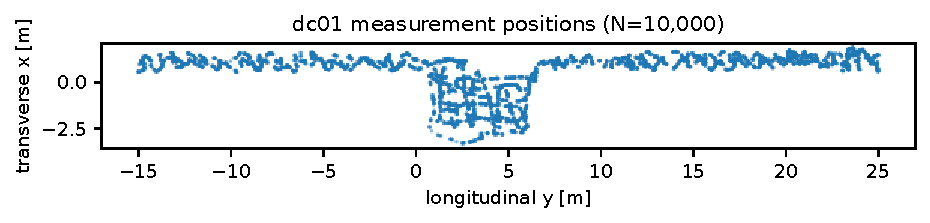
\includegraphics[width=\linewidth,height=0.34\textheight,keepaspectratio]{raw01_dc01_positions_xy.pdf}
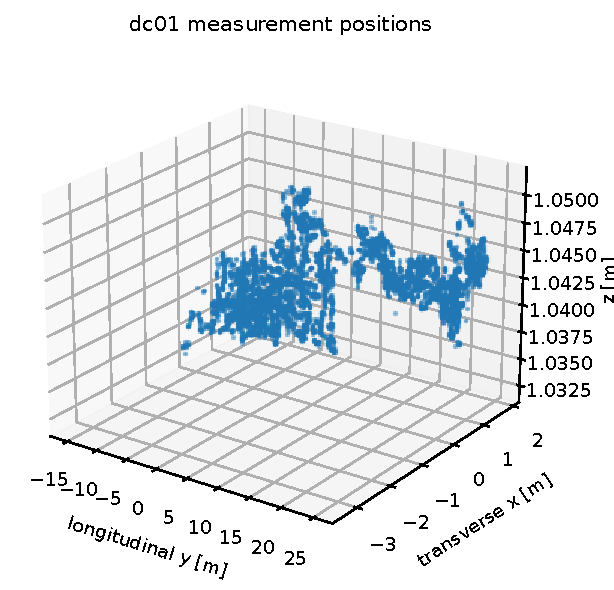
\includegraphics[width=0.62\linewidth,height=0.29\textheight,keepaspectratio]{raw02_dc01_positions_3d.pdf}
\caption{Distribución de las 10,000 posiciones en planta y elevación.}
\end{figure}
\column{0.42\textwidth}
\small
\begin{equation*}
H_i^{\rm real}\in\mathbb C^{2\times32\times1024},
\qquad i=1,\ldots,10{,}000.
\end{equation*}
\begin{itemize}
\item dos arreglos de 32 antenas;
\item 1024 subportadoras sobre $\approx\SI{50}{MHz}$;
\item portadora de \SI{3.438}{GHz};
\item 5000 posiciones de entrenamiento, 100 de validación y 4900 de prueba.
\end{itemize}
Los $640{,}000$ vectores antena--posición comparten captura, escena y referencia de
arreglo. La unidad experimental es la posición, no cada antena.
\end{columns}
\smallsource{Banco DICHASUS dc01; descripción y particiones documentadas en el capítulo experimental del manuscrito.}
\end{frame}

% 5
\begin{frame}{Soporte geométrico de trayectorias}
\begin{columns}[T]
\column{0.58\textwidth}
\begin{figure}
\centering
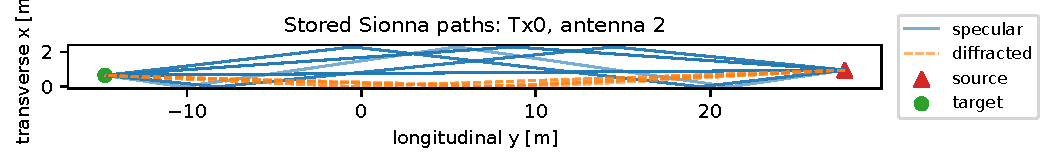
\includegraphics[width=\linewidth,height=0.28\textheight,keepaspectratio]{raw03_sionna_paths_xy.pdf}
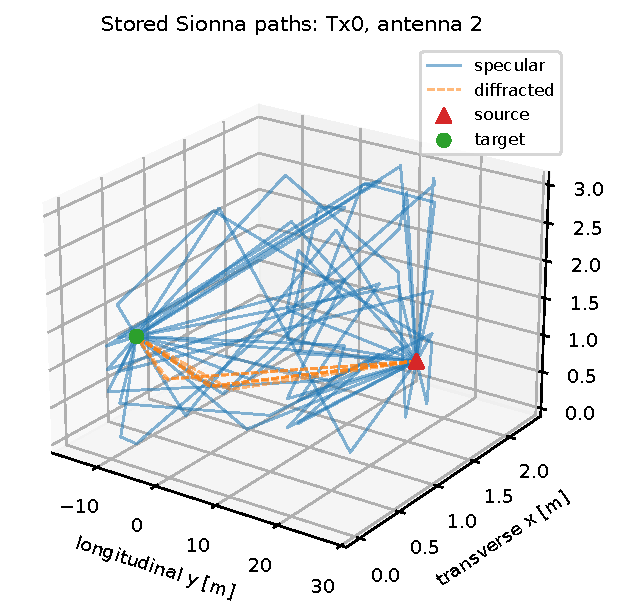
\includegraphics[width=0.52\linewidth,height=0.23\textheight,keepaspectratio]{raw04_sionna_paths_3d.pdf}
\caption{Ejemplo de caminos almacenados para Tx0 y una antena receptora.}
\end{figure}
\column{0.39\textwidth}
\scriptsize
El registro reserva hasta 198 contribuciones especulares, 6 difractadas y 445
difusas por consulta. En B0--B2 se sintetiza
\begin{equation*}
H_{i,u,a}(f_k)=
\sum_{\ell\in\mathcal P_{i,u,a}}
\alpha_{i,u,a,\ell}(f_k)e^{-j2\pi f_k\tau_{i,u,a,\ell}},
\end{equation*}
con \texttt{scattering=False}. La comparación activa utiliza contribuciones
especulares y difractadas; la dispersión difusa almacenada no interviene.
\end{columns}
\conclusion{Las líneas son componentes del modelo directo; no implican que cada camino sea identificable desde la CFR medida.}
\end{frame}

% 6
\begin{frame}{Operador de síntesis común a B0--B2}
\small
Para cada consulta se mantiene fijo el soporte geométrico y se modifica únicamente
la representación material:
\begin{equation*}
H_i^{(b)}=\mathcal S\!\left(\mathcal P_i^{\rm RT},\Theta_b;f_k\right),
\qquad b\in\{0,1,2\}.
\end{equation*}
\vspace{0.12cm}
\begin{center}
\begin{tikzpicture}[>=Latex,node distance=0.45cm,every node/.style={font=\scriptsize}]
\tikzstyle{n}=[draw=navy,thin,minimum width=2.25cm,minimum height=.72cm,align=center,fill=white]
\node[n] (a) {posición y escena};
\node[n,right=of a] (b) {caminos almacenados};
\node[n,right=of b] (c) {campos EM\\$\Theta_b$};
\node[n,right=of c] (d) {CIR\\sin scattering};
\node[n,right=of d] (e) {CFR\\1024 tonos};
\draw[->] (a)--(b);\draw[->] (b)--(c);\draw[->] (c)--(d);\draw[->] (d)--(e);
\end{tikzpicture}
\end{center}
\vspace{0.2cm}
\begin{tabularx}{\textwidth}{p{1.2cm}p{4.6cm}Y}
\toprule
Modelo & Parametrización & Papel experimental\\
\midrule
B0 & Materiales ITU y escala global & Referencia nominal.\\
B1 & $\epsilon_r$ y $\sigma$ constantes por objeto & Calibración paramétrica compartida.\\
B2 & $\epsilon_r(\vect x)$ y $\sigma(\vect x)$ mediante MLP & Heterogeneidad espacial continua.\\
\bottomrule
\end{tabularx}
\end{frame}

% 7
\begin{frame}{B0: referencia nominal}
\begin{figure}
\centering
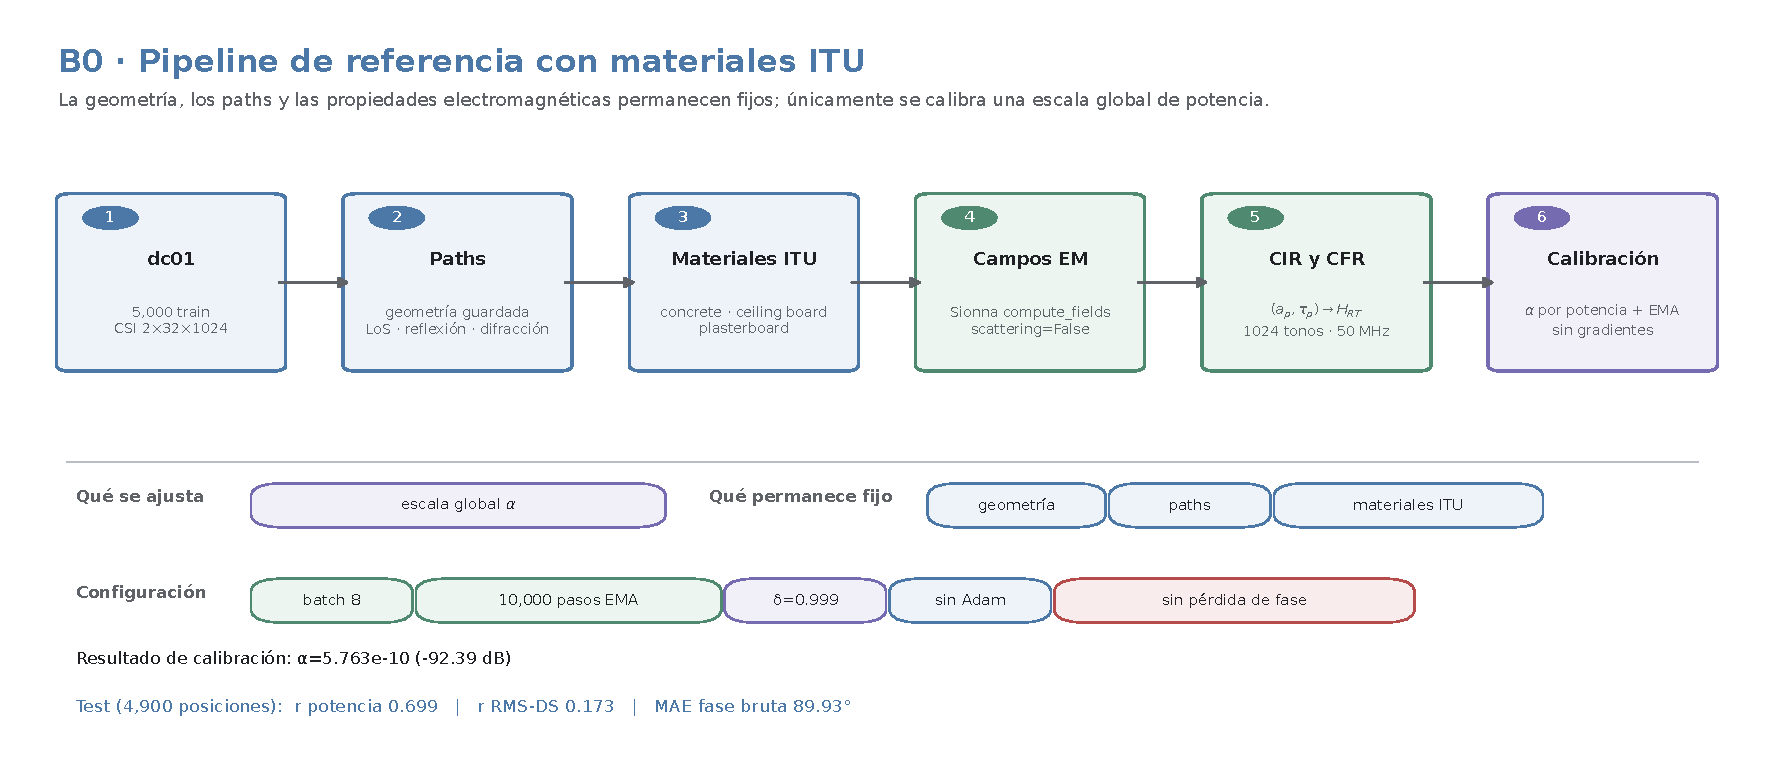
\includegraphics[width=0.94\textwidth,height=0.56\textheight,keepaspectratio]{b0_01_pipeline.pdf}
\caption{Geometría, caminos y materiales ITU permanecen fijos; se estima únicamente la escala global $\alpha$.}
\end{figure}
\end{frame}

% 8
\begin{frame}{B0: calibración de escala}
\begin{columns}[T]
\column{0.58\textwidth}
\begin{figure}
\centering
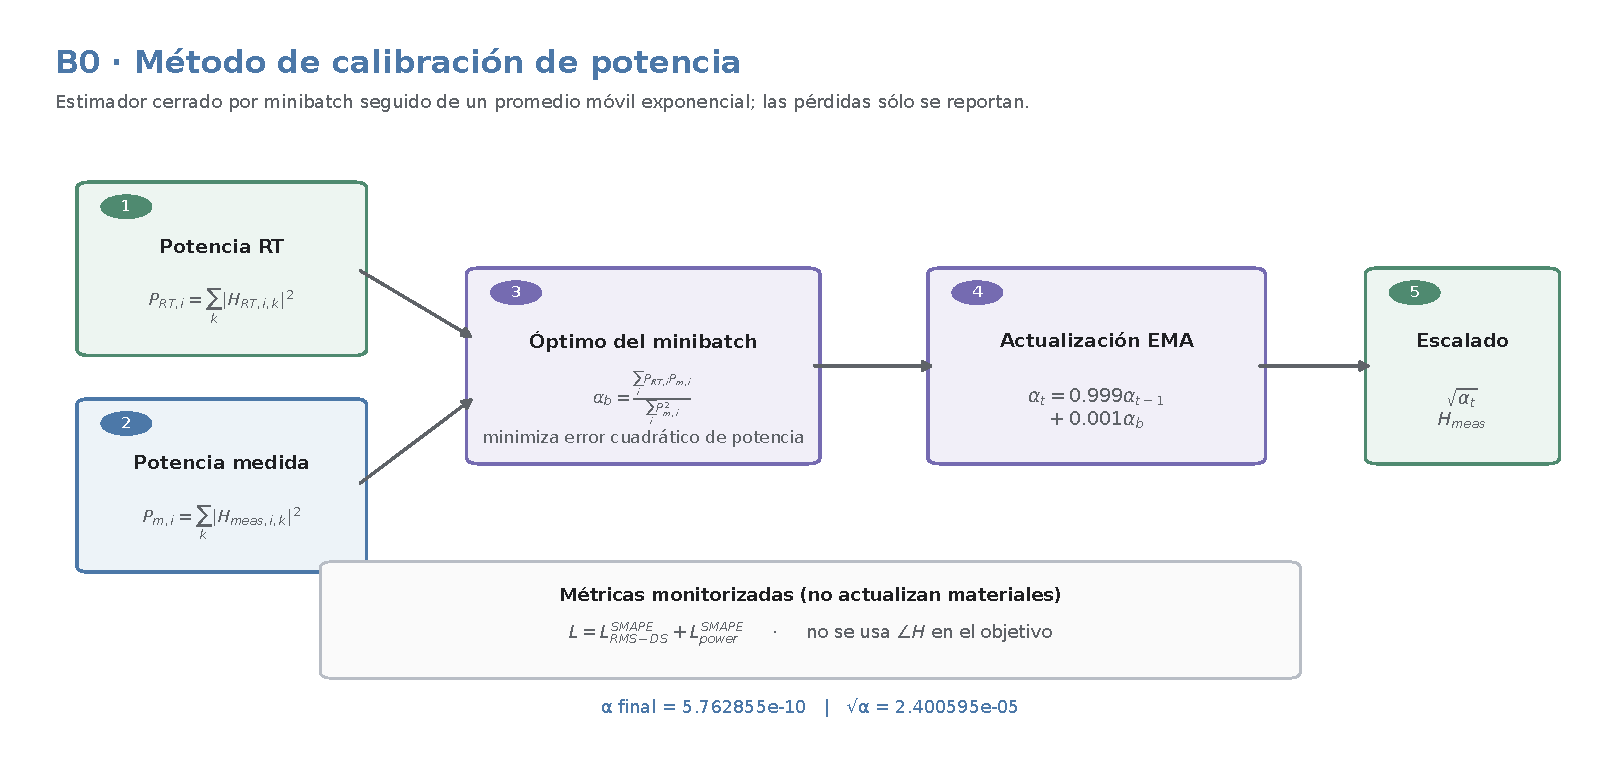
\includegraphics[width=\linewidth,height=0.56\textheight,keepaspectratio]{b0_02_power_scaling.pdf}
\caption{Estimador cerrado por minibatch y actualización EMA.}
\end{figure}
\column{0.39\textwidth}
\scriptsize
\begin{align*}
P_i^{\rm RT}&=\sum_k|H_{i,k}^{\rm RT}|^2,\\
P_i^{\rm real}&=\sum_k|H_{i,k}^{\rm real}|^2,\\
\widehat\alpha_{\mathcal B}&=
\frac{\sum_{i\in\mathcal B}P_i^{\rm RT}P_i^{\rm real}}
{\sum_{i\in\mathcal B}(P_i^{\rm real})^2},\\
\alpha_t&=0.999\alpha_{t-1}+0.001\widehat\alpha_{\mathcal B_t}.
\end{align*}
La ejecución conservada obtiene
\begin{align*}
\alpha&=5.762855\times10^{-10},\\
\sqrt\alpha&=2.400595\times10^{-5}.
\end{align*}
La escala actúa sobre potencia/amplitud y no modifica retardos ni fase relativa.
\end{columns}
\end{frame}

% 9
\begin{frame}{B1: materiales constantes por objeto}
\begin{figure}
\centering
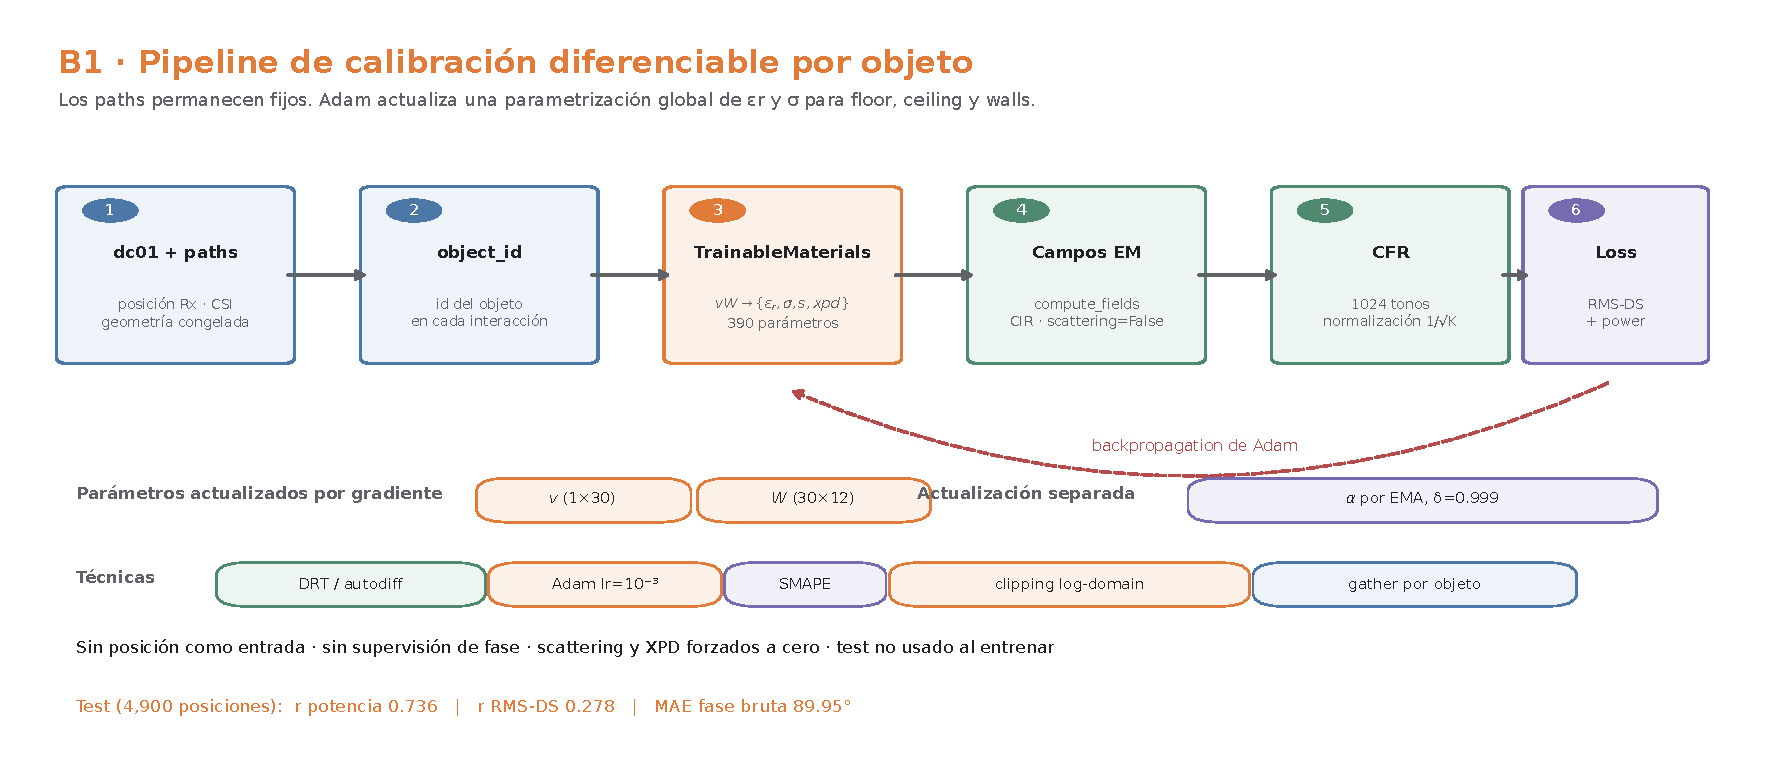
\includegraphics[width=0.94\textwidth,height=0.56\textheight,keepaspectratio]{b1_01_pipeline.pdf}
\caption{Adam actualiza propiedades por objeto a través del trazador diferenciable; los caminos permanecen fijos.}
\end{figure}
\end{frame}

% 10
\begin{frame}{B1: parametrización e identificabilidad}
\begin{columns}[T]
\column{0.58\textwidth}
\begin{figure}
\centering
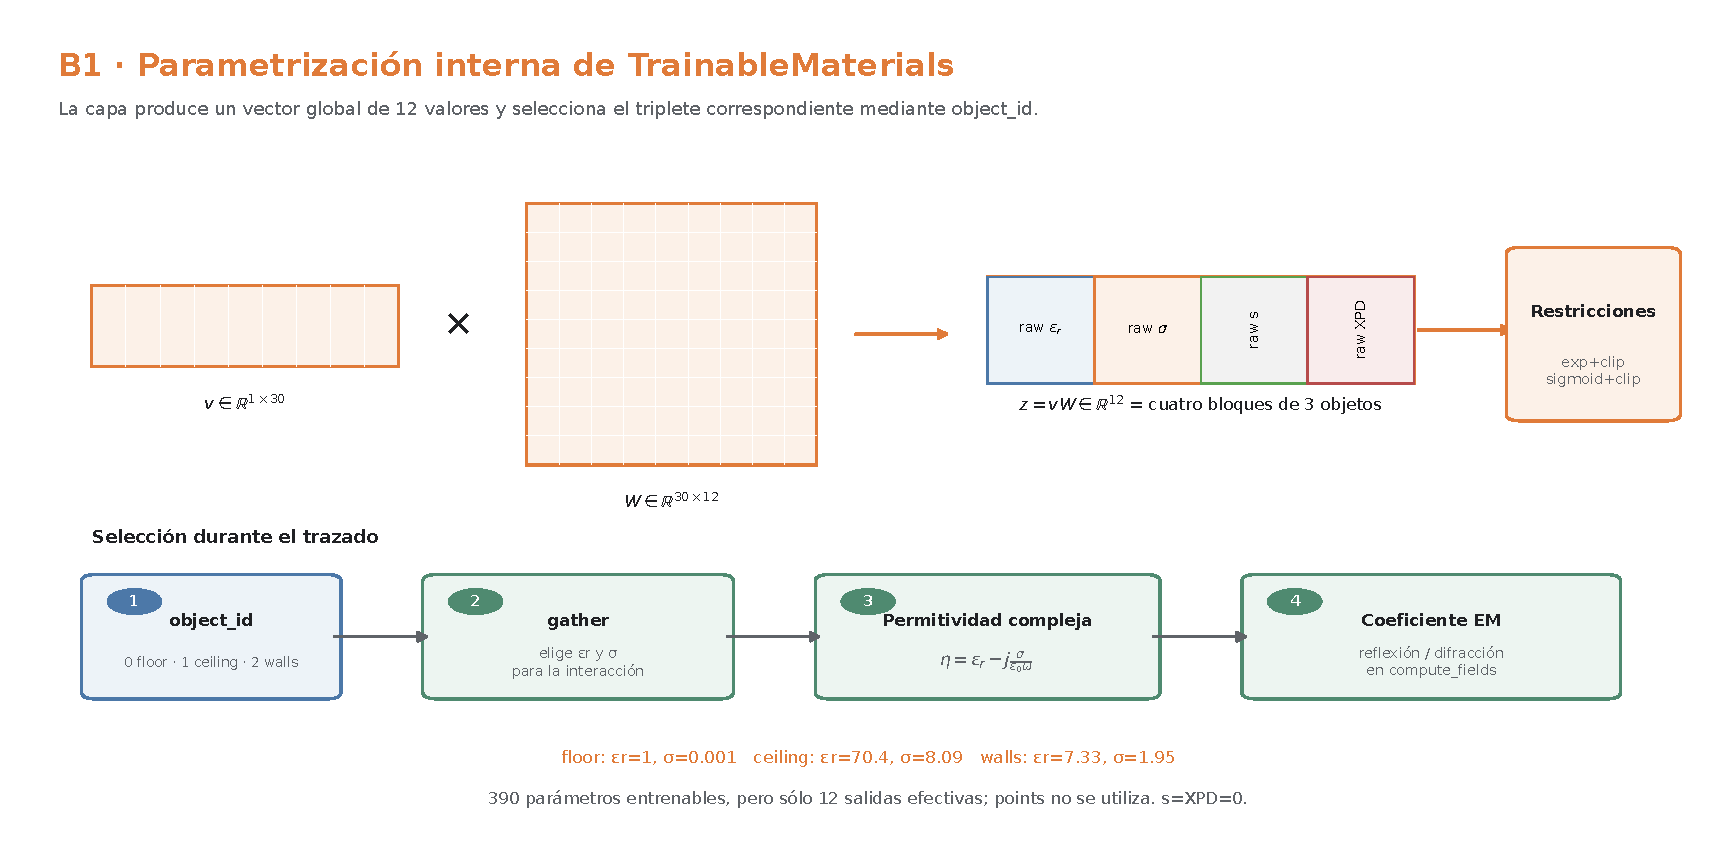
\includegraphics[width=\linewidth,height=0.53\textheight,keepaspectratio]{b1_02_parameterization.pdf}
\caption{Factorización interna y selección mediante identificador de objeto.}
\end{figure}
\column{0.39\textwidth}
\tiny
\begin{align*}
\vect z&=\vect v\vect W\in\mathbb R^{4N_o},\\
\vect v&\in\mathbb R^{1\times30},\qquad
\vect W\in\mathbb R^{30\times4N_o},\\
\epsilon_r&=1+\exp\{\operatorname{clip}(z_\epsilon)\},&
\sigma&=\exp\{\operatorname{clip}(z_\sigma)\}.
\end{align*}
Para $N_o=3$ hay 390 parámetros y 12 salidas; con dispersión y XPD anuladas, sólo
seis cantidades afectan el canal.
\begin{equation*}
\eta_o(f)=\epsilon_{r,o}-j\frac{\sigma_o}{2\pi f\epsilon_0}.
\end{equation*}
Como $(c\vect v)(\vect W/c)=\vect v\vect W$, los factores internos no son
identificables por separado. Los valores aprendidos se interpretan como propiedades
efectivas del modelo.
\end{columns}
\end{frame}

% 11
\begin{frame}{B2: campo neuronal de materiales}
\begin{figure}
\centering
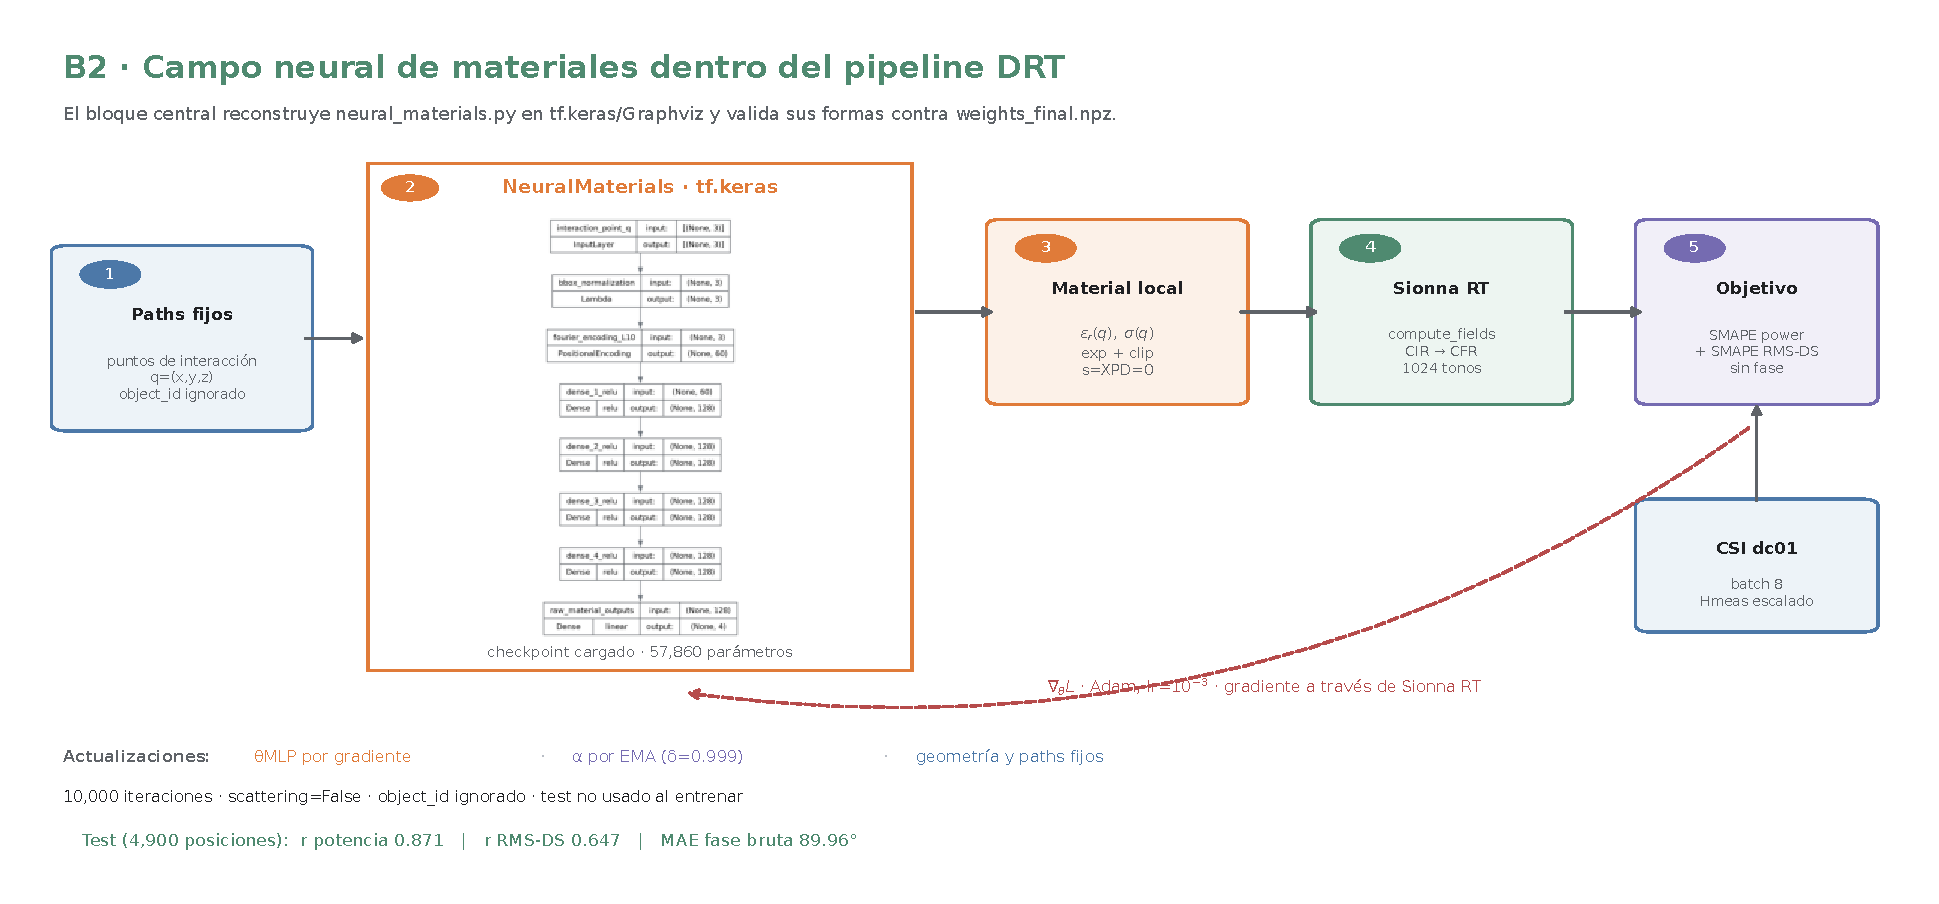
\includegraphics[width=0.94\textwidth,height=0.56\textheight,keepaspectratio]{b2_01_pipeline.pdf}
\caption{La red asigna propiedades locales en los puntos de interacción; la geometría y los caminos no se actualizan.}
\end{figure}
\end{frame}

% 12
\begin{frame}{B2: arquitectura auditada}
\begin{columns}[T]
\column{0.62\textwidth}
\begin{figure}
\centering
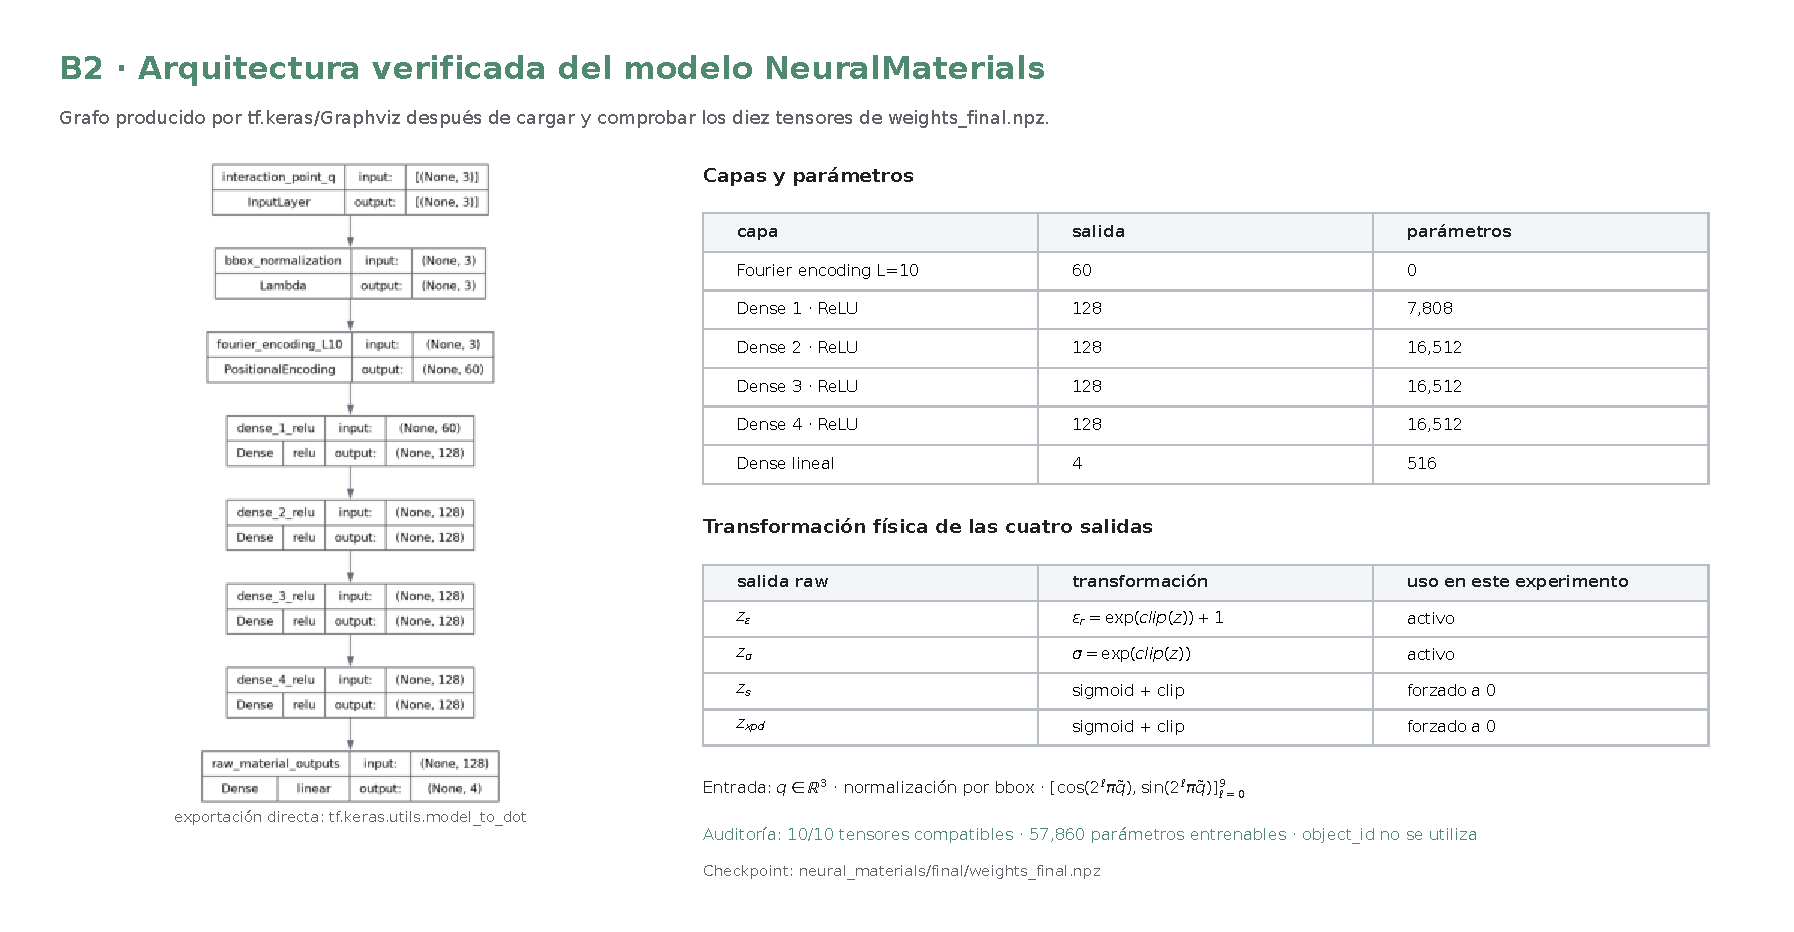
\includegraphics[width=\linewidth,height=0.55\textheight,keepaspectratio]{b2_02_mlp_architecture.pdf}
\caption{Arquitectura verificada contra los tensores del archivo de pesos.}
\end{figure}
\column{0.35\textwidth}
\tiny
La coordenada se normaliza por la caja de la escena y se codifica como
\begin{equation*}
\gamma(\bar{\vect x})=
\left[\cos(2^\ell\pi\bar x_d),\sin(2^\ell\pi\bar x_d)\right]_{
\substack{d=1,2,3\\\ell=0,\ldots,9}}
\in\mathbb R^{60}.
\end{equation*}
Cuatro capas de 128 unidades ReLU y una capa lineal de cuatro salidas contienen
\begin{equation*}
(60\cdot128+128)+3(128\cdot128+128)+(128\cdot4+4)=57{,}860
\end{equation*}
parámetros. Sólo $\epsilon_r(\vect x)$ y $\sigma(\vect x)$ se usan en la síntesis.
\end{columns}
\end{frame}

% 13
\begin{frame}{Objetivo de aprendizaje de B1 y B2}
\small
El protocolo usa Adam con tasa $10^{-3}$, minibatches de ocho consultas y 10,000
iteraciones. La escala $\alpha$ se actualiza fuera de Adam. La pérdida es
\begin{align*}
\mathcal L_b&=\mathcal L_{P,b}+\mathcal L_{\tau,b},\\
\mathcal L_{P,b}&=\frac1N\sum_i
\frac{|P_i^{(b)}-\alpha P_i^{\rm real}|}
{P_i^{(b)}+\alpha P_i^{\rm real}},\\
\mathcal L_{\tau,b}&=\frac1N\sum_i
\frac{|\tau_{{\rm rms},i}^{(b)}-\tau_{{\rm rms},i}^{\rm real}|}
{\tau_{{\rm rms},i}^{(b)}+\tau_{{\rm rms},i}^{\rm real}}.
\end{align*}
\vspace{0.1cm}
\begin{tabularx}{\textwidth}{p{3.1cm}Y}
\toprule
Supervisión explícita & Consecuencia esperable\\
\midrule
Potencia total & Ajuste de escala y variación espacial de energía.\\
RMS delay spread & Ajuste de estructura temporal gruesa.\\
Sin término complejo & No existe presión directa para reconstruir fase absoluta o interferencia fina.\\
\bottomrule
\end{tabularx}
\end{frame}

% 14
\begin{frame}{Resultados consolidados de B0--B2}
\scriptsize
\begin{table}
\centering
\begin{tabular}{lrrr}
\toprule
Métrica & B0 & B1 & B2\\
\midrule
Correlación de potencia $\uparrow$ & 0.699 & 0.736 & \textbf{0.871}\\
MAE de potencia [dB] $\downarrow$ & 6.29 & 3.82 & \textbf{2.22}\\
Correlación RMS-DS $\uparrow$ & 0.173 & 0.278 & \textbf{0.647}\\
MAE RMS-DS [ns] $\downarrow$ & 43.21 & 27.32 & \textbf{16.50}\\
NMSE mediana de magnitud [dB] $\downarrow$ & $-3.17$ & $-3.92$ & \textbf{$-4.46$}\\
Coherencia compleja bruta $\uparrow$ & 0.156 & 0.155 & 0.145\\
Error angular bruto [$^\circ$] $\downarrow$ & 89.93 & 89.95 & 89.96\\
\bottomrule
\end{tabular}
\caption{Evaluación sobre las 4900 posiciones de prueba.}
\end{table}
\vspace{0.1cm}
\conclusion{El aumento de capacidad mejora potencia, magnitud y RMS-DS, pero no induce una mejora de la concordancia compleja.}
\end{frame}

% 15
\begin{frame}{Correspondencia espacial de potencia}
\begin{figure}
\centering
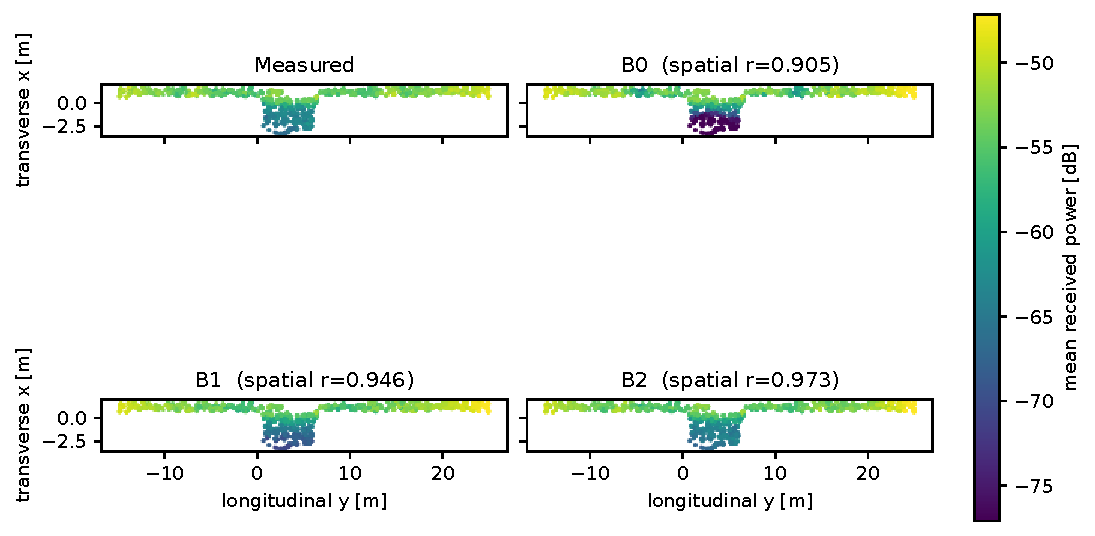
\includegraphics[width=0.94\textwidth,height=0.57\textheight,keepaspectratio]{raw05_spatial_power_maps.pdf}
\caption{Potencia medida y predicha por B0--B2 sobre la región de prueba. B2 reproduce con mayor fidelidad la estructura espacial macroscópica.}
\end{figure}
\end{frame}

% 16
\begin{frame}{CFR medida y simulada}
\begin{figure}
\centering
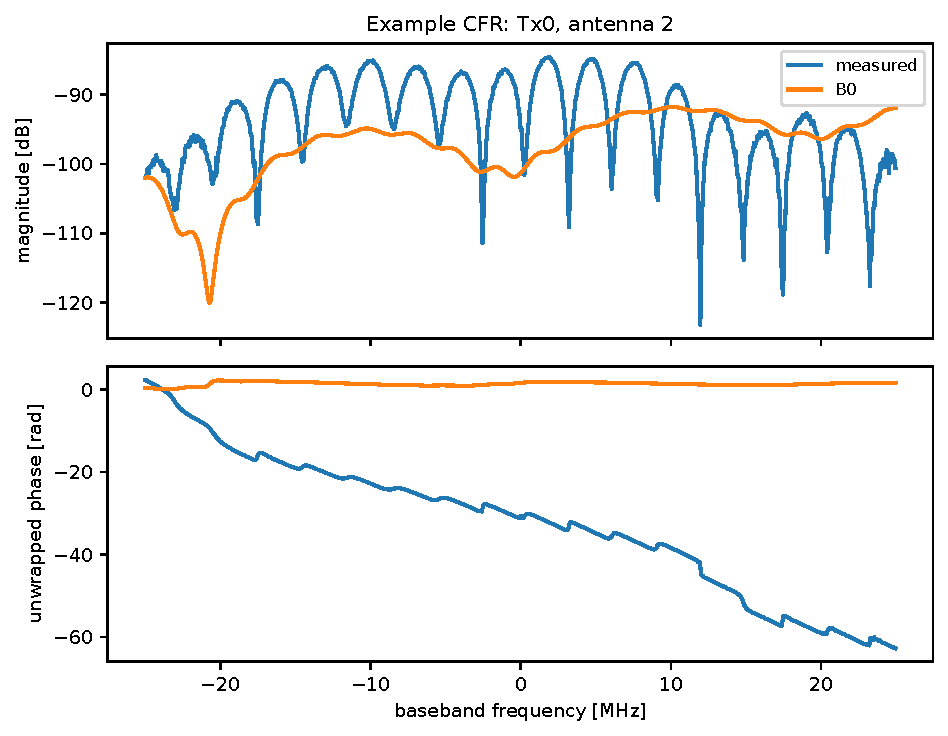
\includegraphics[width=0.92\textwidth,height=0.50\textheight,keepaspectratio]{raw06_cfr_measured_vs_b0.pdf}
\caption{Ejemplo de CFR medida y B0. La envolvente puede ser plausible mientras la interferencia fina y la fase permanecen desalineadas.}
\end{figure}
\conclusion{Una aproximación macroscópica de la envolvente no determina la orientación del vector complejo multifrecuencia.}
\end{frame}

% 17
\begin{frame}{Resumen gráfico de la escalera de capacidad}
\begin{figure}
\centering
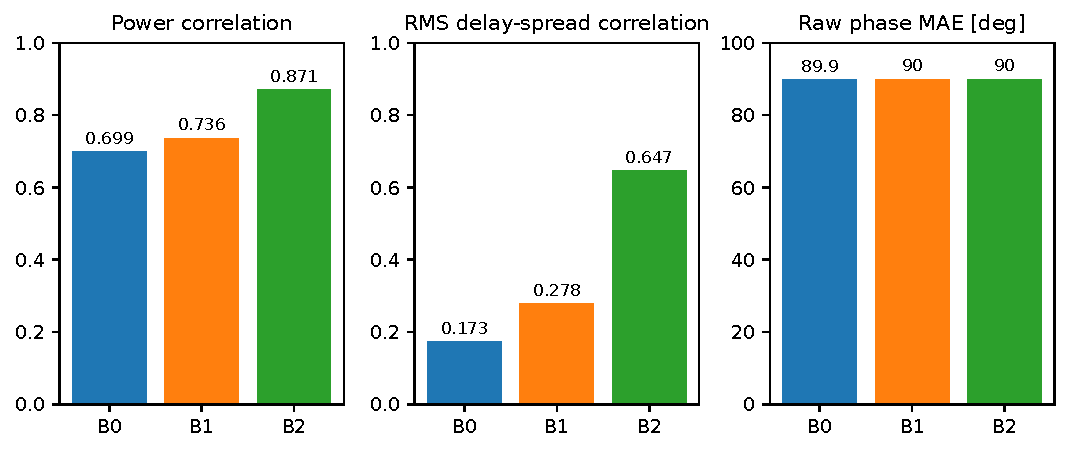
\includegraphics[width=0.88\textwidth,height=0.56\textheight,keepaspectratio]{raw07_b0_b1_b2_metrics.pdf}
\caption{Comparación normalizada de métricas estáticas. La mejora de B2 se concentra en potencia, magnitud y dispersión de retardos.}
\end{figure}
\end{frame}

% 18
\begin{frame}{Construcción progresiva del modelo de discrepancia}
\small
La factorización final se obtuvo mediante una secuencia de contrastes, no mediante
una hipótesis causal fijada de antemano:
\begin{equation*}
\begin{aligned}
\text{B0}&\rightarrow\text{B1--B2}\rightarrow
\text{fallo de fase bruta}\rightarrow\text{residuo complejo}\\
&\rightarrow\text{pendiente espectral}\rightarrow\text{transferencia}
\rightarrow\text{fase común}\rightarrow\text{residuo estructurado}.
\end{aligned}
\end{equation*}
\vspace{0.25cm}
\begin{tabularx}{\textwidth}{p{2.2cm}Y}
\toprule
Etapa & Pregunta sometida a contraste\\
\midrule
S4.1 & ¿Conviene introducir errores circulares independientes por trayectoria?\\
S4.2--S4.3 & ¿Existe estructura agregada de baja dimensión en la discrepancia?\\
S4.4--S4.5 & ¿Puede predecirse sin consultar el canal objetivo en prueba?\\
S4.6 & ¿El intercepto contiene una componente común transferible?\\
\bottomrule
\end{tabularx}
\end{frame}

% 19
\begin{frame}{Sensibilidad de fase a errores geométricos}
\begin{columns}[T]
\column{0.51\textwidth}
\small
Para una trayectoria,
\begin{align*}
H_\ell(f)&=\alpha_\ell(f)e^{-j2\pi f\tau_\ell},\\
\Delta\phi_\ell&=-2\pi f_c\Delta\tau_\ell
=-2\pi\frac{\Delta d_\ell}{\lambda}.
\end{align*}
La longitud de onda fija la sensibilidad angular a desplazamiento, mientras el ancho
de banda fija la capacidad de separar contribuciones en retardo. Son escalas físicas
distintas.
\vspace{0.15cm}
A \SI{25}{MHz} de frecuencia relativa, un error de \SI{2.5}{ns} produce
$22.5^\circ$ de rotación. Esta cifra puede degradar la combinación coherente aun
cuando sea menor que $1/B\approx\SI{20}{ns}$.
\column{0.46\textwidth}
\begin{figure}
\centering
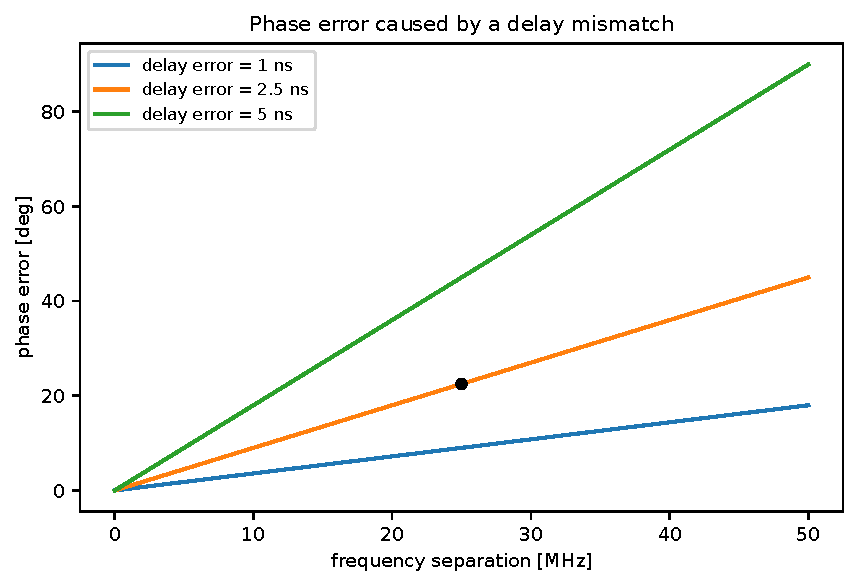
\includegraphics[width=\linewidth,height=0.62\textheight,keepaspectratio]{raw10_phase_sensitivity.pdf}
\caption{Sensibilidad analítica de fase a error temporal.}
\end{figure}
\end{columns}
\end{frame}

% 20
\begin{frame}{S4.1: incertidumbre local de fase}
\small
El modelo de calibración con error local puede escribirse
\begin{equation*}
H^{\rm mod}(f)=\sum_p\alpha_p(f)
\exp\{-j2\pi f\tau_p+j\varepsilon_p\},
\qquad
p(\varepsilon_p|\mu_p,\kappa_p)=
\frac{e^{\kappa_p\cos(\varepsilon_p-\mu_p)}}{2\pi I_0(\kappa_p)}.
\end{equation*}
\begin{tabularx}{\textwidth}{p{1.5cm}p{4.1cm}Y}
\toprule
Método & Supuesto & Consecuencia observada\\
\midrule
PEOC & $\varepsilon_p=0$ & Los materiales pueden absorber discrepancia geométrica.\\
UPEC & fase uniforme & Mayor estabilidad, a costa de descartar estructura angular.\\
PEAC & fase von Mises & Soluciones precisas, con sensibilidad a inicialización y mínimos locales.\\
\bottomrule
\end{tabularx}
\vspace{0.15cm}
La conductividad mostró menor identificabilidad que la permitividad. Antes de
introducir centenares de variables circulares se buscó una representación agregada
de menor dimensión.
\smallsource{Marco metodológico basado en la calibración phase-aware de Ruah et al. y su reproducción experimental.}
\end{frame}

% 21
\begin{frame}{Residuo conjugado e hipótesis afín mínima}
\small
Se define
\begin{equation*}
R_{i,u,a,k}=H^{\rm real}_{i,u,a,k}H^{{\rm RT}*}_{i,u,a,k},
\qquad
\Delta\phi_{i,u,a,k}=\arg R_{i,u,a,k}.
\end{equation*}
Bajo la aproximación
\begin{equation*}
H^{\rm real}_k\simeq c\,e^{-j2\pi\nu_k\Delta\tau}H^{\rm RT}_k+e_k,
\qquad c=|c|e^{j\phi_0},
\end{equation*}
se obtiene
\begin{align*}
R_k&\simeq c\,e^{-j2\pi\nu_k\Delta\tau}|H_k^{\rm RT}|^2,\\
\Delta\phi_k&\simeq\phi_0-2\pi\nu_k\Delta\tau+r_k\pmod{2\pi}.
\end{align*}
El producto evita dividir entre $H^{\rm RT}$ cerca de un nulo y pondera implícitamente
los tonos con energía simultánea en medición y simulación.
\end{frame}

% 22
\begin{frame}{Frecuencia relativa y alineamiento de orden cero}
\small
Con $\nu_k=f_k-f_{\rm ref}$,
\begin{equation*}
-2\pi f_k\Delta\tau=-2\pi f_{\rm ref}\Delta\tau-2\pi\nu_k\Delta\tau.
\end{equation*}
El primer término es constante en frecuencia y se incorpora al intercepto. El CPO se
estima por enlace como
\begin{align*}
\widehat\phi_{{\rm CPO},i,u,a}
&=\arg\left(\sum_{k\in\mathcal K}
H^{\rm real}_{i,u,a,k}H^{{\rm mod}*}_{i,u,a,k}\right),\\
H^{{\rm mod,CPO}}_{i,u,a,k}
&=e^{j\widehat\phi_{{\rm CPO},i,u,a}}H^{\rm mod}_{i,u,a,k}.
\end{align*}
\begin{tabularx}{\textwidth}{p{3.0cm}Y}
\toprule
Grado de libertad & Alcance\\
\midrule
CPO & Rotación constante; alineamiento post hoc si usa el objetivo evaluado.\\
$\Delta\tau_{\rm eff}$ & Pendiente lineal en frecuencia; reorienta la estructura multifrecuencia.\\
$r_k$ & Discrepancia no afín que permanece después de ambos términos.\\
\bottomrule
\end{tabularx}
\end{frame}

% 23
\begin{frame}{Detección de la pendiente y techo oráculo}
\tiny
\renewcommand{\arraystretch}{0.98}
Los incrementos adyacentes eliminan el intercepto:
\begin{equation*}
\arg(R_{k+1}R_k^*)\simeq-2\pi\Delta f\Delta\tau_{\rm eff}.
\end{equation*}
\begin{table}
\centering
\begin{tabular}{lrr}
\toprule
Modelo & Sólo CPO [$^\circ$] & Pendiente adyacente + CPO [$^\circ$]\\
\midrule
B0 & 81.42 & 66.05\\
B1 & 81.39 & 66.48\\
B2 & 81.58 & 54.99\\
\bottomrule
\end{tabular}
\end{table}
El techo global se obtiene mediante
\begin{equation*}
\widehat\tau^{\rm oracle}_{i,u}=
\arg\max_{\tau\in[-500,500]\,{\rm ns}}
\left|\sum_a\sum_k R_{i,u,a,k}e^{j2\pi\nu_k\tau}\right|.
\end{equation*}
\begin{table}
\centering
\begin{tabular}{lrrrr}
\toprule
& \multicolumn{2}{c}{Error angular [$^\circ$]} & \multicolumn{2}{c}{Coherencia}\\
\cmidrule(lr){2-3}\cmidrule(lr){4-5}
Modelo & CPO & Retardo + CPO & Bruta & Retardo + CPO\\
\midrule
B0 & 81.42 & 31.63 & 0.156 & 0.745\\
B1 & 81.39 & 37.15 & 0.155 & 0.696\\
B2 & 81.58 & 38.17 & 0.145 & 0.683\\
\bottomrule
\end{tabular}
\end{table}
\end{frame}

% 24
\begin{frame}{Controles de transferencia del retardo efectivo}
\scriptsize
\begin{tabularx}{\textwidth}{p{3.2cm}p{4.2cm}Y}
\toprule
Control & Resultado & Inferencia permitida\\
\midrule
Entre modelos & $r=0.886$ B0--B1; $0.834$ B0--B2; $0.819$ B1--B2 & La pendiente no depende exclusivamente de una parametrización material.\\
Antenas retenidas & $35.52^\circ$ al transferir; $30.49^\circ$ en antenas usadas & Existe una componente compartida dentro del arreglo.\\
Pares a impares & $31.65^\circ$ & Interpolación intercalada casi conserva el techo.\\
Media banda a media banda & $\approx45^\circ$ & La extrapolación espectral es más difícil.\\
\bottomrule
\end{tabularx}
\vspace{0.3cm}
El retardo efectivo puede reunir error geométrico, centros de fase, trayectorias
ausentes, STO/SFO, cables y respuesta de cadena. El nombre designa la pendiente que
mejor alinea el canal agregado; no identifica una causa física única.
\conclusion{Los controles respaldan una estructura compartida y transferible, pero no una fase absoluta autónoma.}
\end{frame}

% 25
\begin{frame}{Estructura después de retirar pendiente e intercepto}
\begin{columns}[T]
\column{0.58\textwidth}
\begin{figure}
\centering
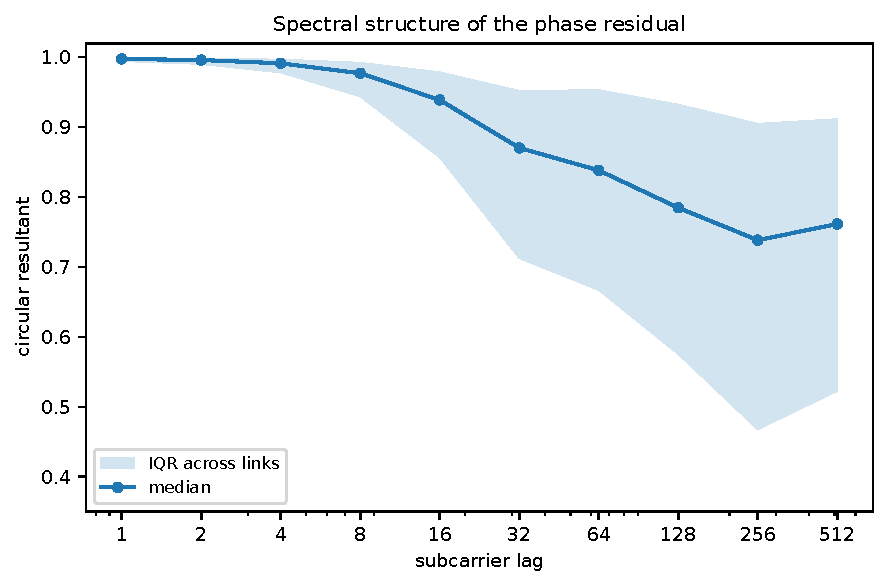
\includegraphics[width=\linewidth,height=0.52\textheight,keepaspectratio]{raw09_phase_residual_structure.pdf}
\caption{Concentración circular del residuo en función de la separación espectral.}
\end{figure}
\column{0.39\textwidth}
\small
\begin{align*}
r_{i,u,a,k}=\operatorname{wrap}\!\bigl(&
\Delta\phi_{i,u,a,k}+2\pi\nu_k\widehat\tau^{\rm oracle}_{i,u}\\
&-\widehat\phi_{0,i,u,a}\bigr).
\end{align*}
Resultados para B0:
\begin{itemize}
\item error angular mediano: $31.63^\circ$;
\item resultante residual mediana: 0.786;
\item incremento adyacente mediano: $2.41^\circ$;
\item concentración $C_1=0.9974$.
\end{itemize}
Una concentración próxima a uno indica regularidad local de los incrementos, no un
residuo de pequeña magnitud.
\end{columns}
\end{frame}

% 26
\begin{frame}{Aprendizaje del retardo efectivo}
\small
La etiqueta de entrenamiento se obtiene con el oráculo; la entrada predictiva no
incluye el canal real de la posición evaluada:
\begin{equation*}
\mathcal D_{\rm train}=
\left\{\left(\vect x_{i,u},y_{i,u}\right)\right\},
\qquad
\vect x_{i,u}=\begin{bmatrix}\vect p_i\\\vect z^{\rm RT}_{i,u}\end{bmatrix}
\in\mathbb R^{51},
\qquad
y_{i,u}=\widehat\tau^{\rm oracle}_{i,u}.
\end{equation*}
Para el árbol $b$, cada partición selecciona variable y umbral por reducción de error:
\begin{equation*}
(j^*,s^*)=\arg\min_{j,s}
\left[
\sum_{n\in\mathcal I_L(j,s)}(y_n-\bar y_L)^2+
\sum_{n\in\mathcal I_R(j,s)}(y_n-\bar y_R)^2
\right].
\end{equation*}
El bosque promedia los regresores construidos sobre muestras bootstrap:
\begin{equation*}
\widehat\tau^{\rm pred}(\vect x)=\frac1T\sum_{b=1}^{T}h_b(\vect x).
\end{equation*}
No se asignan valores de hiperparámetros que no estén documentados en los artefactos
proporcionados.
\end{frame}

% 27
\begin{frame}{Generalización del predictor de retardo}
\scriptsize
\begin{columns}[T]
\column{0.47\textwidth}
\textbf{Partición densa.}\par\vspace{0.1cm}
Bosque con posición y descriptores RT:
\begin{align*}
\mathrm{MAE}&=\SI{10.89}{ns},&
\mathrm{MedAE}&=\SI{4.74}{ns},\\
R^2&=0.867,&
r_{\rm Pearson}&=0.931.
\end{align*}
La distancia mediana al vecino de entrenamiento es \SI{4.83}{cm}; el resultado
caracteriza principalmente interpolación densa.
\column{0.49\textwidth}
\textbf{Cinco bloques espaciales.}\par\vspace{0.1cm}
Cada bloque contiene 2000 posiciones y se impone una guarda de \SI{0.5}{m}.
\begin{table}
\centering
\begin{tabular}{lr}
\toprule
Entrada & MAE [ns]\\
\midrule
Posición & 27.56\\
Descriptores RT & 19.29\\
Posición + RT & \textbf{18.69}\\
\bottomrule
\end{tabular}
\end{table}
Los descriptores RT aportan información regional más allá de copiar coordenadas
próximas.
\end{columns}
\conclusion{La evidencia es intraescena y la variable objetivo conserva el significado operativo del oráculo.}
\end{frame}

% 28
\begin{frame}{Aplicación del retardo predicho al canal}
\begin{columns}[T]
\column{0.57\textwidth}
\begin{figure}
\centering
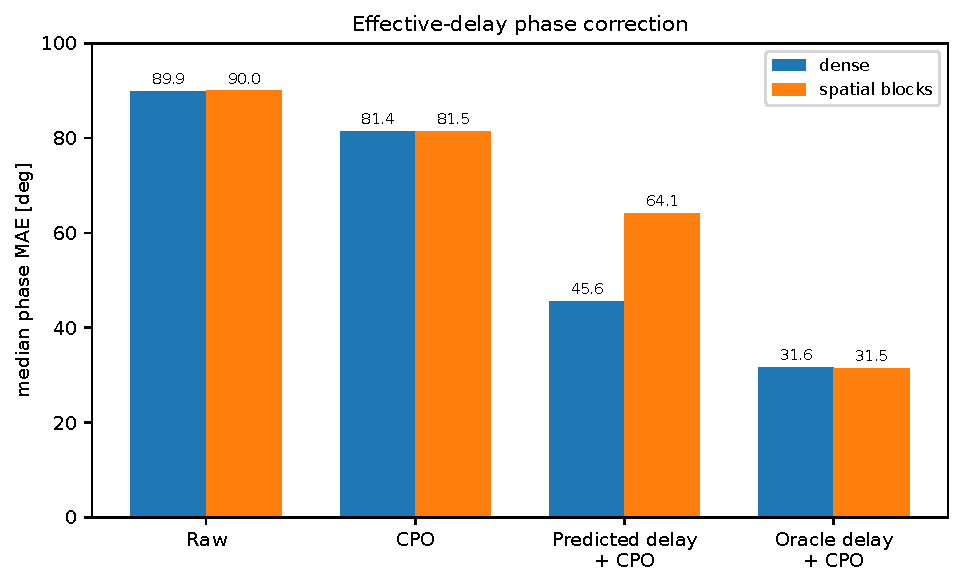
\includegraphics[width=\linewidth,height=0.50\textheight,keepaspectratio]{raw08_phase_correction.pdf}
\caption{MAE angular de B0 bajo partición densa y espacialmente bloqueada.}
\end{figure}
\column{0.40\textwidth}
\small
\begin{equation*}
H^{{\rm RT,corr}}_{i,u,a,k}=H^{\rm RT}_{i,u,a,k}
\exp\{-j2\pi\nu_k\widehat\tau^{\rm pred}_{i,u}\}.
\end{equation*}
\begin{tabular}{lrr}
\toprule
Protocolo & Error [$^\circ$] & $\rho$\\
\midrule
Denso, CPO & 81.42 & 0.156\\
Denso, pred. & 45.59 & 0.634\\
Bloques, CPO & 81.49 & 0.157\\
Bloques, pred. & 64.08 & 0.448\\
\bottomrule
\end{tabular}
\vspace{0.15cm}
La coherencia
\begin{equation*}
\rho=\frac{|\vect h^H\widehat{\vect h}|}
{\|\vect h\|_2\|\widehat{\vect h}\|_2}
\end{equation*}
es invariante a CPO. Su mejora proviene de la corrección dependiente de frecuencia.
\end{columns}
\end{frame}

% 29
\begin{frame}{Fase común al arreglo y factorización final}
\scriptsize
El intercepto por enlace se descompone descriptivamente como
\begin{equation*}
\phi_{0,i,u,a}\simeq\beta_{u,a}+\psi_{i,u}+\epsilon_{i,u,a}\pmod{2\pi}.
\end{equation*}
Las resultantes por antena son pequeñas (0.01024 en Tx0 y 0.00630 en Tx1). Dentro
de una captura, la resultante mediana es 0.4216; retirar $\psi$ reduce
$88.99^\circ$ a $45.97^\circ$, pero usa las mismas antenas evaluadas. Vecinos
espaciales y temporales no muestran predictibilidad transferible.
\vspace{0.1cm}
La organización resultante es
\begin{equation*}
\boxed{\begin{aligned}
\Delta\phi_{i,u,a,k}\simeq{}&
-2\pi\nu_k\Delta\tau_{{\rm eff},i,u}\\
&+\psi_{i,u}+r^{\rm rel}_{i,u,a,k}\pmod{2\pi}
\end{aligned}}
\end{equation*}
con $r^{\rm rel}=\beta+\epsilon+r_\phi$.
\begin{table}
\centering
\begin{tabularx}{\textwidth}{p{2.0cm}p{5.0cm}Y}
\toprule
Componente & Evidencia & Papel metodológico\\
\midrule
$\Delta\tau_{\rm eff}$ & Transferencia parcial espacial, espectral y entre antenas & Predecir y validar fuera de muestra.\\
$\psi$ & Dirección común a posteriori, sin regla local predictiva & Referenciar, medir o marginalizar.\\
$r^{\rm rel}$ & Suavidad espectral y relación con distribución energética & Modelar con estructura y abstención.\\
\bottomrule
\end{tabularx}
\end{table}
\end{frame}

% 30
\begin{frame}{Representaciones relativas e identificabilidad pathwise}
\scriptsize
\begin{columns}[T]
\column{0.56\textwidth}
\textbf{S4.7-R: discriminabilidad espacial.}
\begin{table}
\centering
\begin{tabular}{lrrr}
\toprule
Métrica & RT bruto & RT+$\widehat\tau$ & Cambio\\
\midrule
Victoria global & 0.5913 & 0.7957 & 0.2044\\
Victoria local & 0.5200 & 0.5560 & 0.0360\\
Mismo bloque & 0.5888 & 0.8872 & 0.2984\\
Entre bloques & 0.6652 & 0.9440 & 0.2788\\
Top-1 & 0.048 & 0.156 & 0.108\\
\bottomrule
\end{tabular}
\end{table}
IC95\% global: $[0.1801,0.2281]$; local: $[-0.0016,0.0732]$. La mejora local no
es concluyente.
\column{0.40\textwidth}
\textbf{S4.7-Ub.0: inversión por trayectorias.}
\begin{table}
\centering
\begin{tabular}{lrr}
\toprule
Caso & $\kappa(G)$ & $\mu_{\max}$\\
\midrule
Tx0 & $2.79\times10^2$ & 0.997073\\
Tx1 & $1.45\times10^6$ & 0.999974\\
\bottomrule
\end{tabular}
\end{table}
El rango algebraico completo coexiste con columnas casi indistinguibles. Las
ecuaciones normales agravan la condición y ridge introduce sesgo.
\end{columns}
\conclusion{La representación relativa mejora discriminabilidad regional estática; no demuestra todavía sensibilidad a movimiento.}
\end{frame}

% 31
\begin{frame}{Dominio de validez de la evidencia}
\scriptsize
\begin{tabularx}{\textwidth}{p{4.0cm}Y}
\toprule
Condición & Consecuencia inferencial\\
\midrule
Una escena dc01 & No demuestra transferencia entre edificios.\\
\SI{3.438}{GHz} y $\approx\SI{50}{MHz}$ & No se extrapola automáticamente a Wi-Fi, LoRa o mmWave.\\
10,000 posiciones estáticas & No contiene movimiento fisiológico ni mecánico.\\
64 antenas y 1024 subportadoras & Un dispositivo COTS puede perder apertura o soporte espectral.\\
Dispersión difusa desactivada & El residuo puede contener mecanismos de propagación omitidos.\\
Retardo oráculo como etiqueta & La variable aprendida no identifica una causa física única.\\
CPO ajustado con el objetivo & El error angular completo sigue siendo condicional.\\
$\psi$ estimada con las mismas antenas & La reducción de fase común es descriptiva.\\
Sin reinicios estacionarios & No se separan PLL, reloj y estado de cadena RF.\\
Sin ground truth dinámico & No puede afirmarse recuperación de forma de onda.\\
\bottomrule
\end{tabularx}
\vspace{0.2cm}
La hipótesis que permanece abierta es si una representación con mejor correspondencia
compleja estática conserva también la perturbación inducida por movimiento.
\end{frame}

% 32
\begin{frame}{De fidelidad estática a fidelidad diferencial}
\begin{columns}[T]
\column{0.48\textwidth}
\small
Alrededor de un estado $q_0$,
\begin{align*}
H(f,q_0+\Delta q)&\simeq H(f,q_0)+J_q(f;q_0)\Delta q,\\
J_q(f;q_0)&=\left.\frac{\partial H(f,q)}{\partial q}\right|_{q=q_0}.
\end{align*}
Se distinguen dos errores:
\begin{align*}
e_0&=H^{\rm real}(q_0)-H^{\rm RT}(q_0),\\
e_J&=J_q^{\rm real}-J_q^{\rm RT}.
\end{align*}
Un modelo puede reducir $e_0$ sin reducir $e_J$. Para sensado, $e_J$ determina si
la dirección y amplitud de la perturbación están bien representadas.
\column{0.49\textwidth}
\begin{figure}
\centering
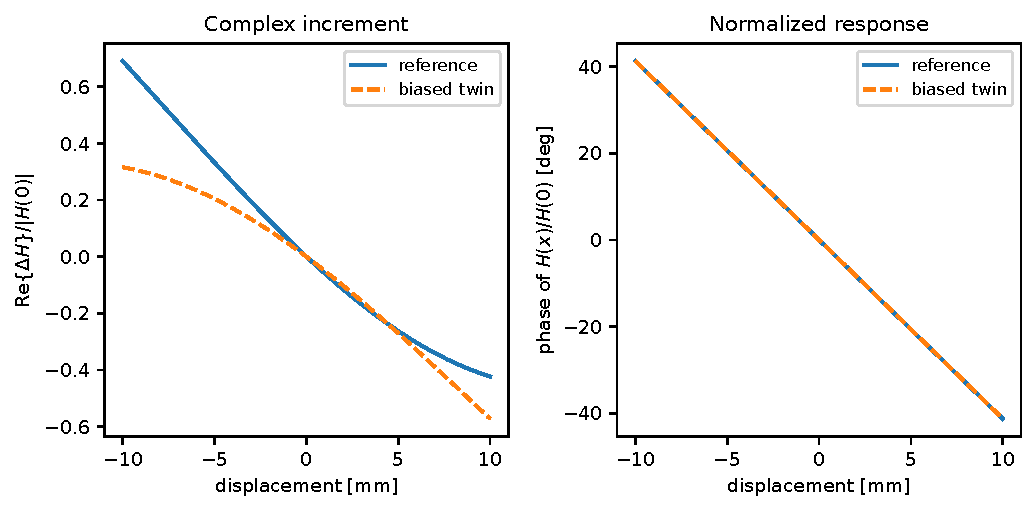
\includegraphics[width=\linewidth,height=0.61\textheight,keepaspectratio]{raw11_differential_fidelity.pdf}
\caption{Coincidencia estática frente a coincidencia de la respuesta diferencial.}
\end{figure}
\end{columns}
\end{frame}

% 33
\begin{frame}{Sensibilidad, nuisance y métrica final}
\small
Para una observación compleja gaussiana con media $\vect\mu(q)$ y covarianza
$\Sigma$, la información local es
\begin{equation*}
F_q=2\operatorname{Re}\left\{J_q^H\Sigma^{-1}J_q\right\}.
\end{equation*}
Si $\zeta$ reúne ganancia, CPO o retardo instrumental, la información equivalente es
\begin{equation*}
F_{q|\zeta}=F_{qq}-F_{q\zeta}F_{\zeta\zeta}^{\dagger}F_{\zeta q}.
\end{equation*}
\begin{tabularx}{\textwidth}{P{2.9cm}P{4.0cm}Y}
\toprule
Nivel & Métricas & Pregunta\\
\midrule
Comunicación & RSSI, SNR, PER/BER & ¿El enlace transporta información?\\
Perturbación & SSNR, SCR, fracción dinámica & ¿El movimiento supera ruido y fondo estático?\\
Sensibilidad & $\|J_q\|$, $F_{q|\zeta}$, CRLB & ¿El estado es observable después de nuisance?\\
Tarea & correlación, NRMSE, lag, morfología & ¿Se recuperó $q(t)$ contra ground truth?\\
\bottomrule
\end{tabularx}
\end{frame}

% 34
\begin{frame}{Patrón fisiológico objetivo y criterio de tarea}
\begin{columns}[T]
\column{0.67\textwidth}
\begin{figure}
\centering
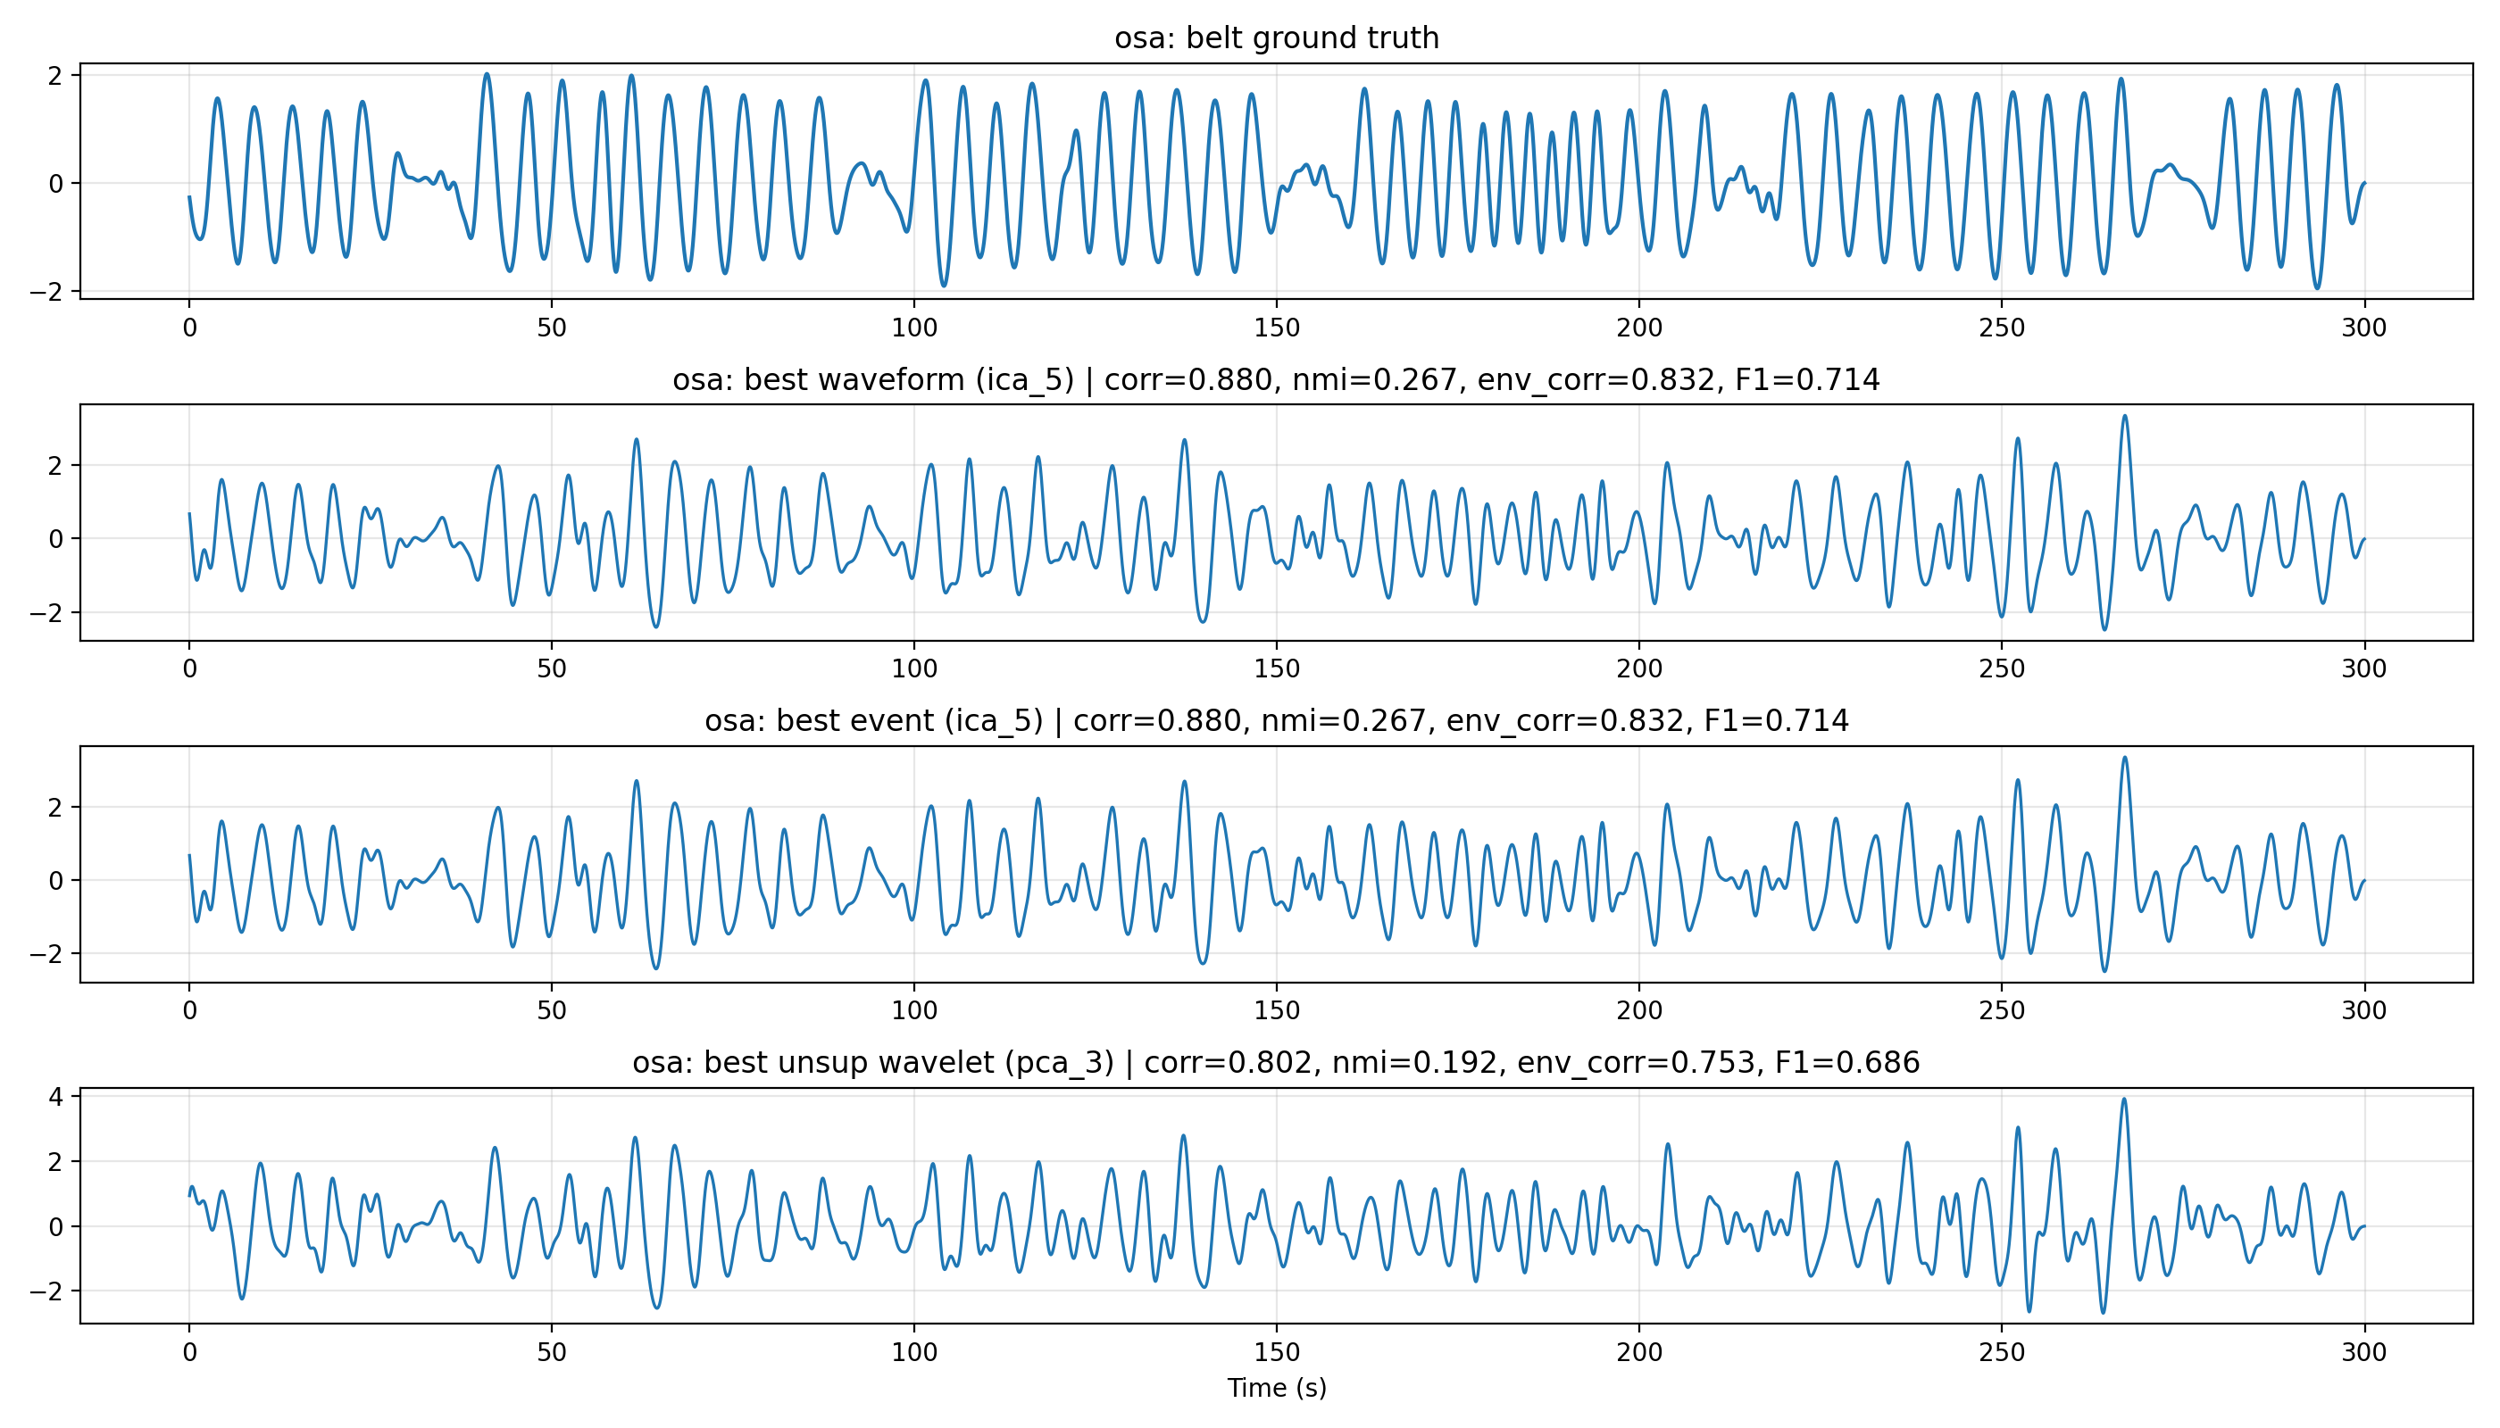
\includegraphics[width=\linewidth,height=0.54\textheight,keepaspectratio]{osa_waveforms.png}
\caption{Referencia de cinturón y reconstrucciones conservadas del análisis OSA.}
\end{figure}
\column{0.30\textwidth}
\scriptsize
La forma de onda de referencia define una evaluación de tarea que exige conservar
morfología, sincronía y eventos. En el artefacto mostrado, el componente ICA
seleccionado reporta
\begin{align*}
r&=0.880, & r_{\rm env}&=0.832,\\
F_1&=0.714.&&
\end{align*}
mientras que la alternativa wavelet no supervisada alcanza $r=0.802$ y
$F_1=0.686$.

Estos valores pertenecen al análisis fisiológico mostrado y no constituyen evidencia
de validación del gemelo digital RF.
\end{columns}
\conclusion{La validación RF debe culminar en métricas contra ground truth temporal, después de demostrar fidelidad diferencial con movimiento controlado.}
\end{frame}

% 35
\begin{frame}{Validación propuesta con movimiento mecánico conocido}
\small
\begin{center}
\begin{tikzpicture}[>=Latex,node distance=.7cm,every node/.style={font=\scriptsize}]
\tikzstyle{n}=[draw=navy,thin,minimum width=2.05cm,minimum height=.7cm,align=center]
\node[n] (tx) {Tx\\Wi-Fi / LoRa};
\node[n,right=of tx] (target) {reflector móvil\\$q_{\rm GT}(t)$};
\node[n,right=of target] (rx) {Rx\\CSI / IQ};
\node[n,right=of rx] (jet) {Jetson\\adquisición};
\node[n,above=.62cm of target] (gt) {radar + cámara\\+ comparador};
\node[n,below=.62cm of target] (act) {etapa lineal\\+ controlador};
\draw[->] (tx)--(target);\draw[->] (target)--(rx);\draw[->] (rx)--(jet);
\draw[->] (gt)--(target);\draw[->] (act)--(target);
\draw[->,dashed] (gt.east) to[bend left=15] (jet.north);
\draw[->,dashed] (act.east) to[bend right=15] (jet.south);
\end{tikzpicture}
\end{center}
\vspace{0.15cm}
Para una trayectoria biestática de longitud
$L(q)=\|\vect q-\vect p_T\|+\|\vect q-\vect p_R\|$,
\begin{equation*}
\frac{\partial L}{\partial q}=
\widehat{\vect u}_T+\widehat{\vect u}_R,
\qquad
\frac{\partial\phi}{\partial q}=-\frac{2\pi}{\lambda}
(\widehat{\vect u}_T+\widehat{\vect u}_R)^T\vect d.
\end{equation*}
La dirección $\vect d$ no debe fijarse sin análisis: se propone una orientación de
alta sensibilidad y otra próxima a nulo como control geométrico.
\end{frame}

% 36
\begin{frame}{Instrumentación y metrología}
\scriptsize
\begin{columns}[T]
\column{0.49\textwidth}
\textbf{Infraestructura disponible}
\begin{itemize}
\item Jetson Orin Nano para adquisición y marcas temporales.
\item Cámara binocular calibrada y LiDAR MS200.
\item Medidor láser y estructura rígida de aluminio.
\item IWRL6432BOOST como referencia independiente.
\item PlutoSDR y NUCLEO-WL55 para LoRa.
\item Router/ESP32 para CSI Wi-Fi, sujeto a extracción compleja estable.
\item Sensores de temperatura y humedad, cuando estén disponibles.
\end{itemize}
\column{0.49\textwidth}
\textbf{Elementos por incorporar}
\begin{itemize}
\item Etapa lineal micrométrica con 25--50 mm de recorrido.
\item Actuador guiado o NEMA 17 con husillo T8.
\item ESP32/Arduino y controlador TMC2209.
\item Comparador digital con salida de datos.
\item Placa de aluminio de $20\times20$ cm y reflectores intercambiables.
\item Soportes rígidos y marcas ChArUco/AprilTag.
\end{itemize}
\end{columns}
\vspace{0.18cm}
{\color{rulegray}\rule{\textwidth}{0.45pt}}
\vspace{0.1cm}
Un canal LoRa de 125 kHz no reproduce el análisis de pendiente de dc01 sobre 50 MHz.
En LoRa se evaluará principalmente la evolución temporal de amplitud y fase/IQ.
\end{frame}

% 37
\begin{frame}{Protocolo de excitación y adquisición}
\scriptsize
\begin{columns}[T]
\column{0.48\textwidth}
\textbf{Secuencia de movimiento}
\begin{enumerate}
\item reposo durante cinco minutos;
\item posiciones estáticas: 0, 1, 2, 5 y 10 mm;
\item sinusoides de 2, 5 y 10 mm;
\item frecuencias de 0.1, 0.2, 0.3 y 0.5 Hz;
\item inspiración rápida, espiración lenta y pausas;
\item amplitud variable y movimiento grueso superpuesto;
\item repetición después de reiniciar Tx y Rx;
\item dos o tres posiciones y dos orientaciones geométricas.
\end{enumerate}
Cada condición se repite al menos cinco veces.
\column{0.49\textwidth}
\textbf{Variables sincronizadas}
\begin{itemize}
\item CSI complejo Wi-Fi o IQ LoRa;
\item posición ordenada y posición medida del actuador;
\item radar, cámara y comparador;
\item timestamps y eventos de reinicio;
\item CFO, RSSI, SNR y configuración del receptor;
\item temperatura, humedad y poses de Tx/Rx/reflector.
\end{itemize}
Las particiones se realizan por repetición y posición. Ventanas del mismo ensayo no
se distribuyen entre entrenamiento y prueba como réplicas independientes.
\end{columns}
\end{frame}

% 38
\begin{frame}{Comparación y criterios de avance}
\small
Todas las representaciones se evalúan sobre la misma adquisición, partición y señal
mecánica de referencia:
\begin{equation*}
\left\{|H|,\;H,\;HH_{\rm ref}^*,\;\text{productos antena/frecuencia},\;
\widehat\tau^{\rm pred},\;\widehat\tau^{\rm oracle}\right\}.
\end{equation*}
\begin{tabularx}{\textwidth}{p{3.4cm}Y}
\toprule
Salida & Métricas\\
\midrule
Forma de onda $\widehat q(t)$ & correlación, NRMSE, lag y DTW.\\
Morfología por ciclo & amplitud, duración inspiración/espiración y pausas.\\
Contenido espectral & error de frecuencia y coherencia espectral.\\
Robustez & degradación tras reinicio, cambio de posición y cambio de orientación.\\
\bottomrule
\end{tabularx}
\vspace{0.2cm}
El criterio para avanzar a sujetos es recuperar consistentemente movimientos de
1--5 mm y patrones respiratorios artificiales, con incertidumbre y tasa de fallas
declaradas. La reducción de error angular estático no constituye por sí sola un
criterio de éxito.
\end{frame}

% 39
\begin{frame}{Conclusiones}
\small
\begin{enumerate}
\setlength\itemsep{0.22cm}
\item B1 y B2 mejoran potencia, magnitud y RMS-DS porque esas cantidades intervienen
en la función objetivo; la coherencia compleja bruta no mejora.
\item La discrepancia de fase contiene una pendiente espectral unidimensional que se
transfiere parcialmente entre modelos, antenas, frecuencias y regiones.
\item Un Random Forest predice parte de ese retardo desde posición y descriptores RT;
la evaluación bloqueada reduce la mejora respecto de la partición densa.
\item La fase común presenta estructura dentro de captura, pero no predictibilidad
local demostrada con las covariables evaluadas.
\item El residuo conserva suavidad espectral y no debe modelarse como ruido angular
independiente ni como una fase libre por trayectoria sin análisis de resolubilidad.
\item La siguiente contribución debe establecer si estas representaciones preservan
$\partial H/\partial q$ y mejoran la reconstrucción de movimiento conocido.
\end{enumerate}
\end{frame}

% 40
\begin{frame}{Referencias principales}
\footnotesize
\begin{thebibliography}{9}
\bibitem{Molisch}
A. F. Molisch, \emph{Wireless Communications: From Fundamentals to Beyond 5G}, 3rd ed., Wiley, 2022.
\bibitem{Sionna}
J. Hoydis et al., ``Sionna RT: Differentiable Ray Tracing for Radio Propagation Modeling,'' 2023.
\bibitem{Calibration}
J. Hoydis et al., ``Learning Radio Environments by Differentiable Ray Tracing,'' 2024.
\bibitem{Ruah}
F. Ruah et al., ``Calibrating Wireless Ray Tracing for Digital Twinning Using Local Phase Error Estimates,'' 2024.
\bibitem{DICHASUS}
M. Euchner et al., ``DICHASUS: A Distributed Channel Sounder Dataset,'' 2023.
\bibitem{Breiman}
L. Breiman, ``Random Forests,'' \emph{Machine Learning}, vol. 45, pp. 5--32, 2001.
\bibitem{Directional}
K. V. Mardia and P. E. Jupp, \emph{Directional Statistics}, Wiley, 2000.
\end{thebibliography}
\vspace{0.15cm}
La bibliografía completa y las claves exactas se conservan en el manuscrito y en
\texttt{references.bib}.
\end{frame}

\end{document}
